\documentclass[a4paper,12pt]{article}
\usepackage{graphicx}
\begin{document}

\vspace*{\fill}
\centerline{\huge \textbf{Documentation}} \hspace*{\fill}
\vspace*{\fill}
\\
\tableofcontents
\newpage

\section{Introduction}
This web application is a forum of questions and answers, akin to \emph{stackoverflow} and \emph{yahoo answers}. The web service will let a user find solutions to problems either by browsing the web site or asking a question oneself. Questions can be answered by other users and each answer can be rated. Highest rated solution offers are shown at the top. With enough questions and answers in the database, the service can provide a quick and convenient way to look up a solution for a problem of any kind. Tags can be added to the asked question to help browsing questions by category.\\
\indent Service will be hosted on university's users-server via Tomcat. Code will be written in Java via NetBeans IDE. App will use PostgreSQL database. User's browser will not require other scripts or plug-ins.
\newpage

\section{General view of the application}
The following is an actor chart, followed with a description for each user and action.\\
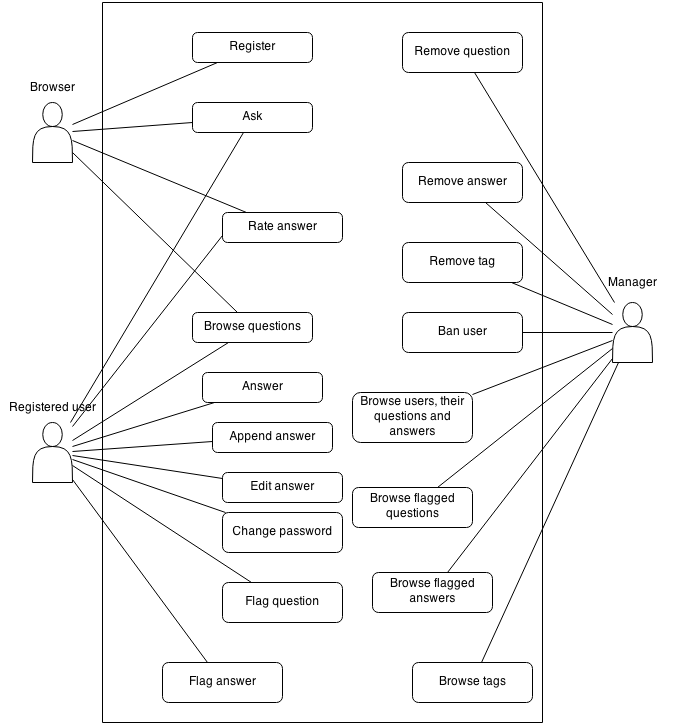
\includegraphics[scale=0.6]{ActorChart}

\noindent \textbf{Browser:} Unregistered user, that got access to the webapp simply by retrieving an url-link.\\
\textbf{Registered user:} User that has access to exclusive features by creating an account and logging into the app.\\
\textbf{Manager:} Webapp manager obligated to managing the forum, keeping it accessible to other users.\\

\noindent User actions:\\
\\
\textbf{Register:} Browser creates an account and promotes oneself into a registered user. User can then login to that account at any time if not banned.\\
\textbf{Ask:} User creates a question, awaiting a set of answers. Also sets tags for the question to improve the transparency of the question.\\
\textbf{Rate answer:} User marks answer as helpful and correct. Answer variant with most ratings is shown on top.\\
\textbf{Browse questions:} Lists questions by tags, (possibly a search function).\\
\textbf{Answer:} Adds an answer to a specified question.\\
\textbf{Append answer:} User edits one's answer by adding information into it. This way of editing will retain the rating of the answer.\\
\textbf{Edit answer:} User edits one's answer freely. This will reset the rating for the answer.\\
\textbf{Change password:} Registered user changes one's password.\\
\textbf{Flag question:} Notifies manager that specified question is inappropriate.\\
\textbf{Flag answer:} Notifies manager that specified answer is inappropriate.\\
\\
\textbf{Remove question:} Removes the specified question along with its answers.\\
\textbf{Remove answer:} Removes the specified answer.\\
\textbf{Remove tag:} Removes a tag from the database.\\
\textbf{Ban user:} Removes the user from the database. Questions and answers made by the user are either marked as 'banned', or removed completely.\\
\textbf{Browse users, their questions and answers}\\
\textbf{Browse flagged questions:} Lists questions by their amount of flags. Helps finding inappropriate questions.\\
\textbf{Browse flagged answers:} Lists answers by their amount of flags. Helps finding inappropriate answers.\\
\textbf{Browse tags:} Lists tags. Whether they are inappropriate or not is apparent directly from the tag.\\
\newpage

\section{System's datacontents}
The following is a chart representing the required data contents of the system on a conceptual level:\\
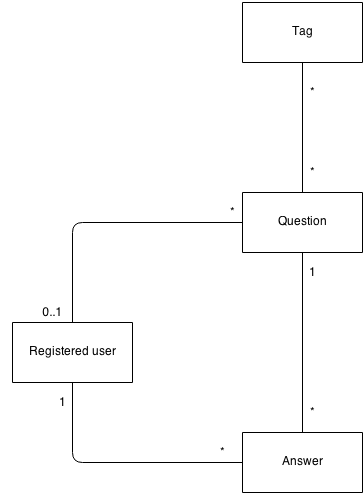
\includegraphics{ConceptChart}
\newpage
\noindent Four datablocks shown in the chart have following properties:\\
\\
\textbf{Datablock: Registered user}
\begin{center}
    \begin{tabular}{ | p{4cm} | p{3cm} | p{5cm} |}
    \hline
    Property & Value interval & Description \\ \hline
    Nickname/Username & 16 characters & User's calling name in the forum. Can't be empty. \\ \hline
    E-mail & 64 characters & User's email to contact one. Can be omitted. \\ \hline
    Password & 128 characters & User's password to access the account. Can't be empty. \\
    \hline
    Time user registered the account & Date and time &  \\
    \hline
    Avatar & 512x512 sized picture & User's picture to identify him by. Can be omitted. \\
    \hline
    \end{tabular}
\end{center}
\hspace*{\fill}\\
\textbf{Datablock: Question}
\begin{center}
    \begin{tabular}{ | p{4cm} | p{3cm} | p{5cm} |}
    \hline
    Property & Value interval & Description \\ \hline
    Question title & 96 characters & Question's essence displayed in search results. Can't be empty \\ \hline
    Question body & Any amount of text & Main part of the question. \\ \hline
    Time when question was asked & Date and time &  \\
    \hline
    Amount of flags for the question & Integer starting from 0 & How many times question was deemed by users as inappropriate. Questions with most flags are easier for a manager to find. \\
    \hline
    \end{tabular}
\end{center}
\hspace*{\fill}\\
\textbf{Datablock: Tag}
\begin{center}
    \begin{tabular}{ | p{4cm} | p{3cm} | p{5cm} |}
    \hline
    Property & Value interval & Description \\ \hline
    Tag title & 12 characters & Can't be empty \\ \hline
    Time when tagged & Date and time & Time when tag was first used. \\ \hline
    \end{tabular}
\end{center}
\newpage
\textbf{Datablock: Answer}
\begin{center}
    \begin{tabular}{ | p{4cm} | p{3cm} | p{5cm} |}
    \hline
    Property & Value interval & Description \\ \hline
    Answer body & Any amount of text &  \\ \hline
    Rating & Integer starting from 0 & Amount of positive points other users have given to this answer. \\ \hline
    Amount of flags for the answer & Integer starting from 0 & How many times answer was deemed by users as inappropriate. Answers with most flags are easier for a manager to find. \\
    \hline
    Approved by asker & Boolean & True if poster of the question which this answer addresses has rated this answer. \\
    \hline
    Time when answer was posted & Date and time & This value is reset if answer is edited. \\
    \hline
    Time when answer was last edited & Date and time & This value is reset if new information is appended to the answer. \\
    \hline
    \end{tabular}
\end{center}
User can post multiple questions and answers. Each question and answer belongs to one user, although question may be posted anonymously, that way it won't belong to any user. Question may contain several answers. Each answer belongs to one question. Question may contain several tags and several question may be tagged with the same tag.
\newpage

\section{Relation data base chart}
\hspace*{\fill}\\
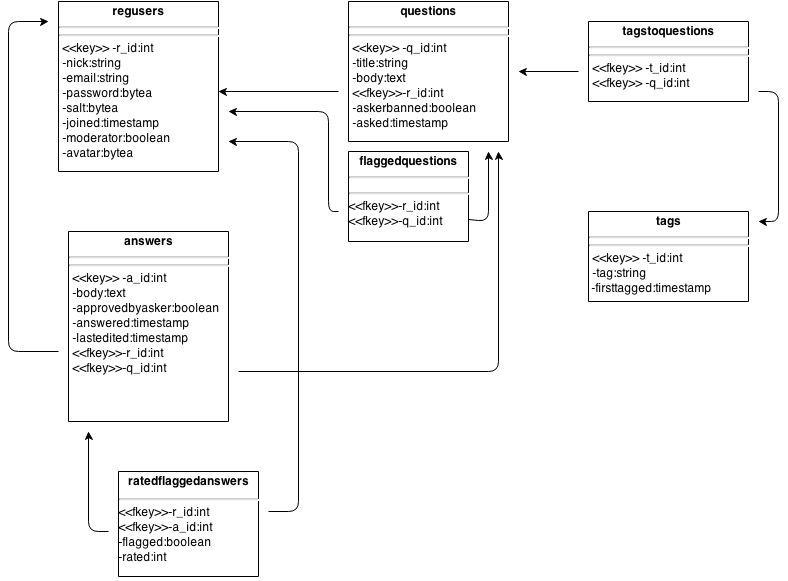
\includegraphics[scale=0.5]{RelationalDBChart}
\newpage

\section{User interface}
The following is a map which represents all the sites that are accessible in the application, and what sites user can access next from the specified site:\\
\\
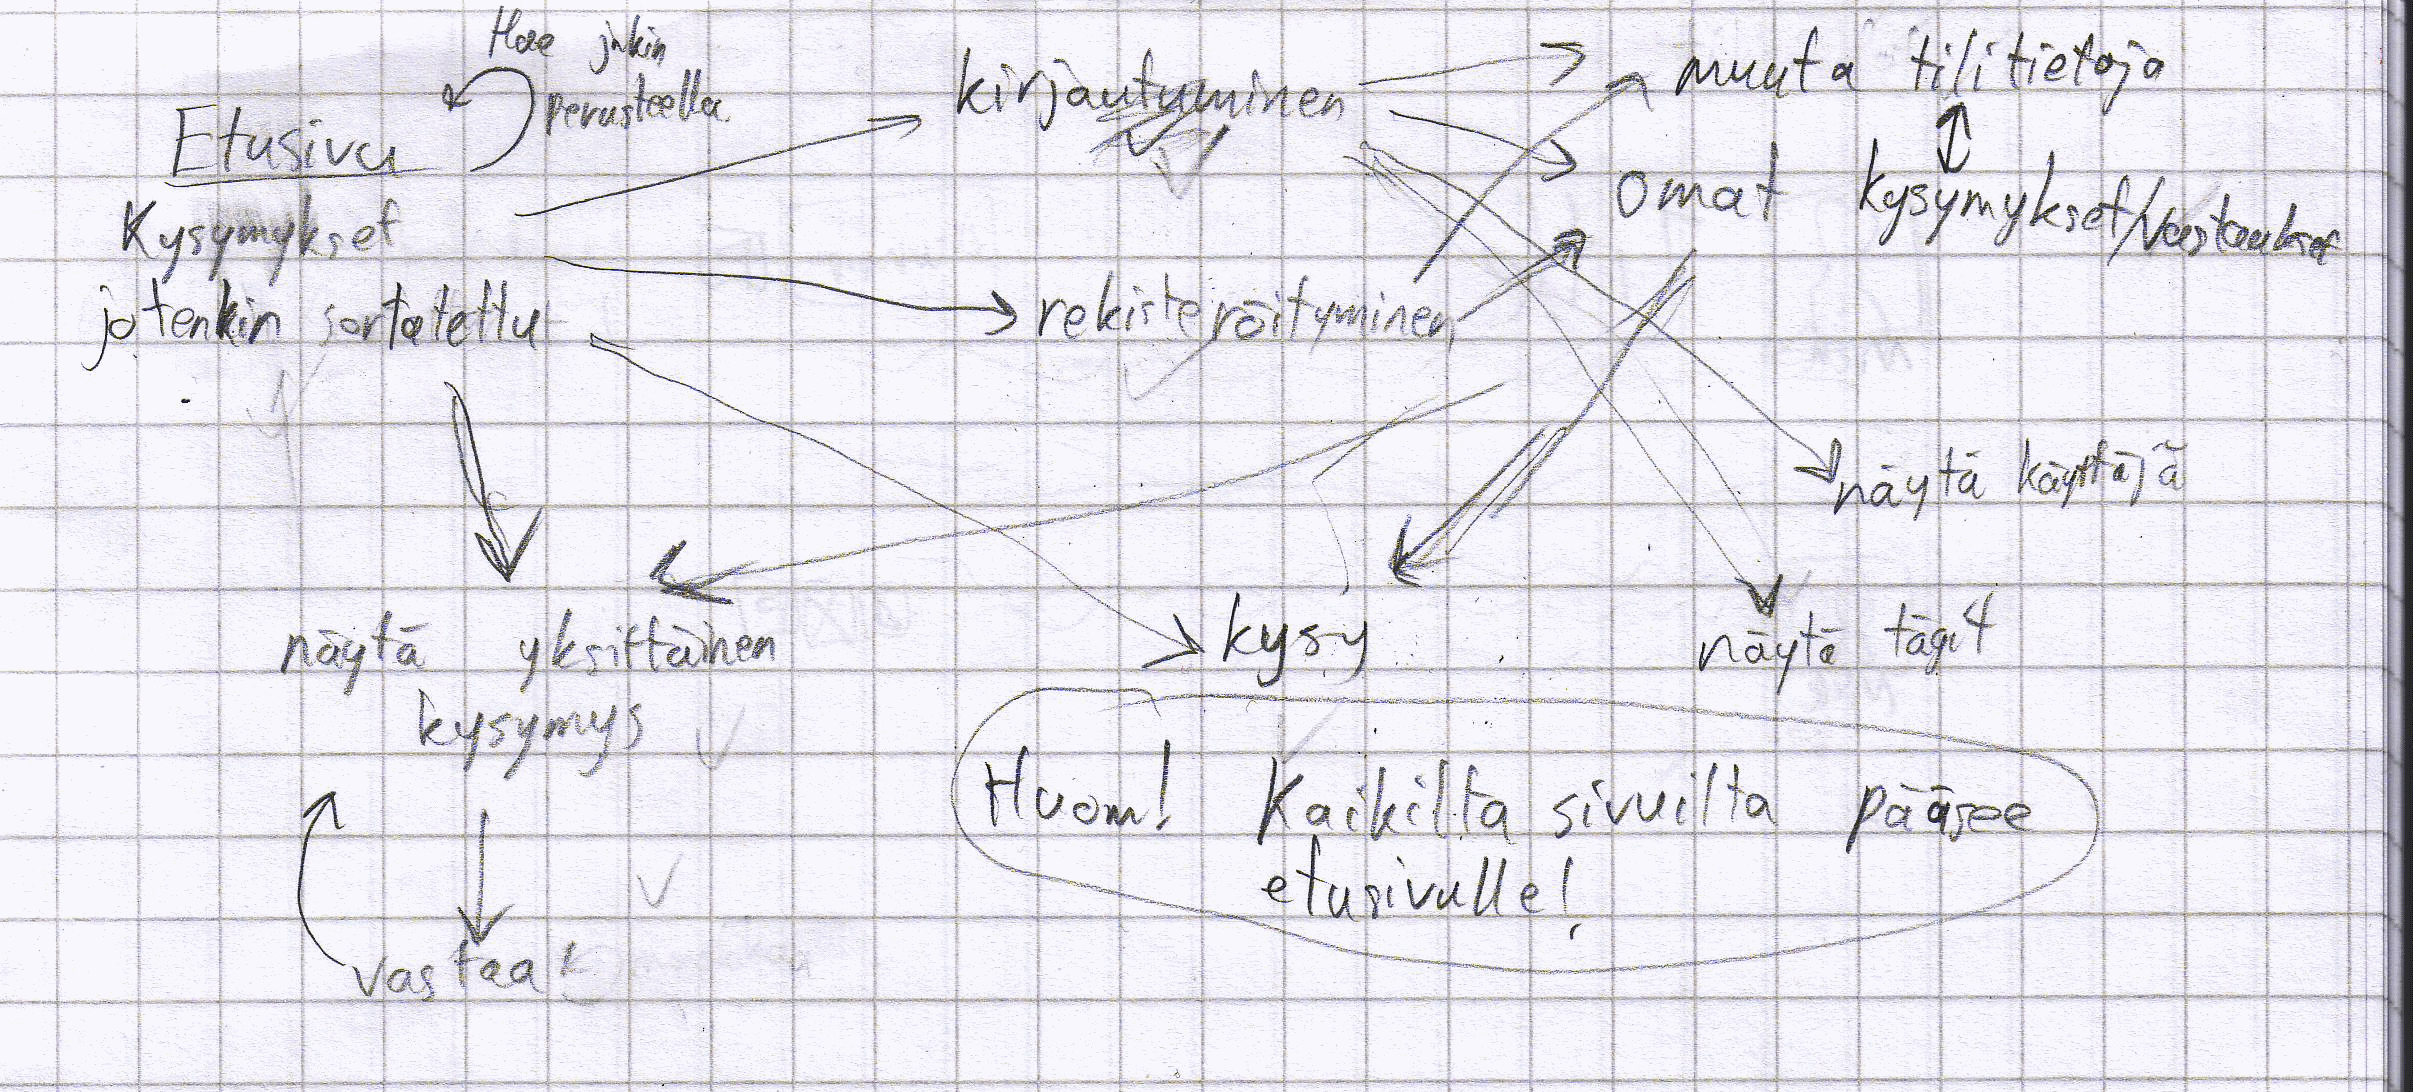
\includegraphics[scale=0.7]{sitemap}\\
\\
This is a design concept of the front page. Notice that it lists asked questions, offers user to ask a question, sign in or register.\\
\\
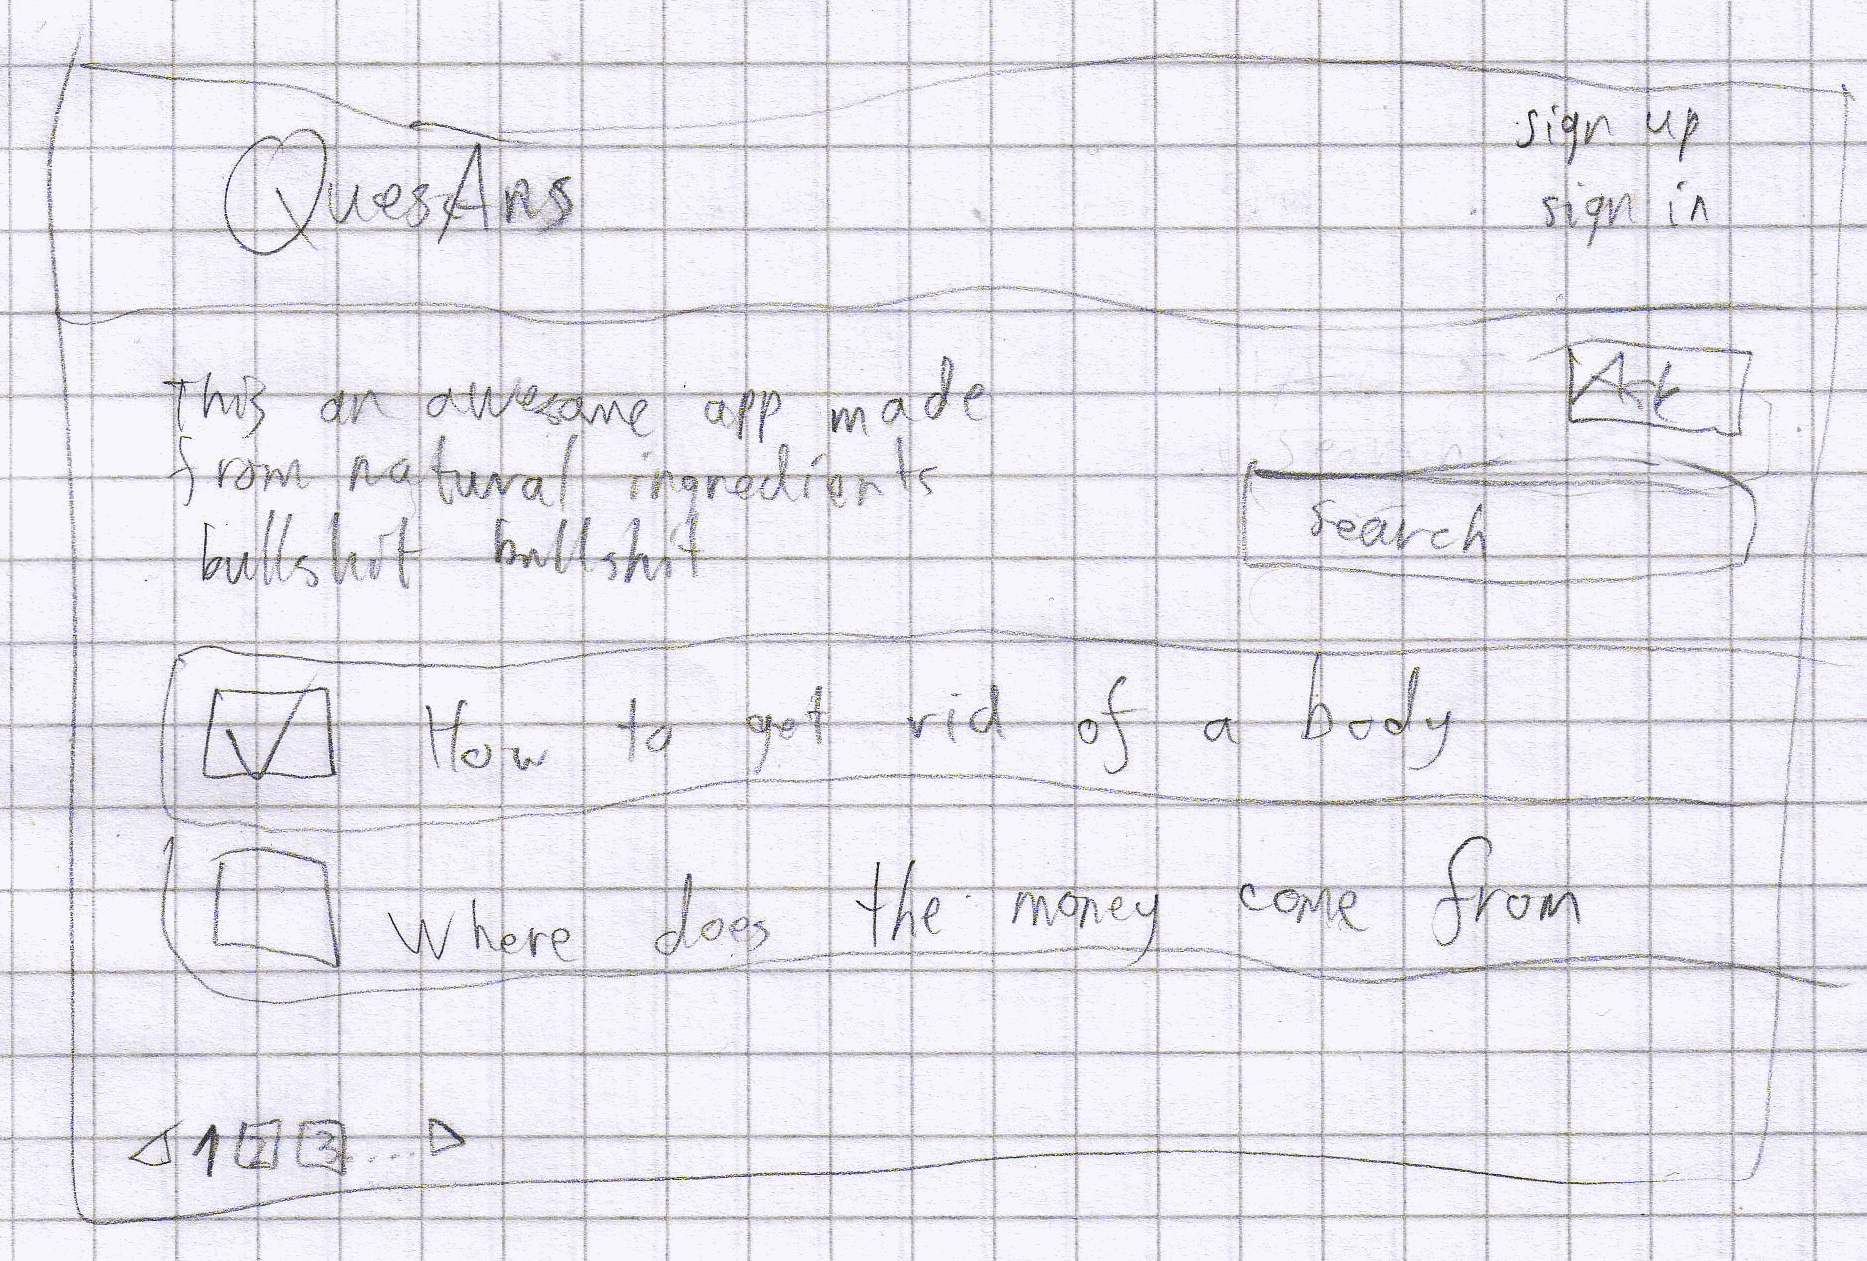
\includegraphics[scale=0.9]{FrontPage}

\end{document}